% ============================================================================
\section{Numerical evidence}\label{sec:numerics}
% ============================================================================
\emph{Everything in this section is numerical evidence and is not used in any proof.}

\paragraph{Method.} Discretized nonlinear programs were solved by multistart interior point (CasADi/IPOPT). For M1 the
discretization is \emph{inner}: $b$ is piecewise geodesic with node-to-node angle at most $\omega h$, and $d_k$ must lie within
$\delta$ of both $b_k$ and $b_{k+1}$. Spherical caps are geodesically convex, so every discrete solution is an admissible
continuous-time trajectory, and every reported distance to a reachable set is an \emph{upper} bound on the true one.
Multistart cannot certify global optima, and ``no gap found'' is weak evidence. Models: M1 (planar and 3-D, with coning
initial guesses), M1A (angular-acceleration-limited axis), M3 (torque-coupled TVC rigid body, quaternion attitude, gimbal
rate $100^\circ$/s), and MT (tilt-angle-rate only, azimuth free). Parameters are those of the motivating vehicle: $m_0=80$~kg,
$T\in[400,1000]$~N, $\alpha=5.66\times10^{-4}$~s/m, $\delta=15^\circ$, $J_\perp=63.6$~kg\,m$^2$, $L=0.589$~m, and
$\omega=0.4$~rad/s in the state-constrained studies. A Mars-like parameter set after \cite{acikmese2007jgcd} was also used.

\subsection{Theorem B regime: gap law and the ball bound}
For $t_f=2$~s, $\omega=30^\circ$/s, $\delta=15^\circ$, the midpoint $M$ lies $2.18$--$2.23$~m/s from $R$, converging in $N$
(\cref{fig:Rsection}). 3-D controls gain essentially nothing over planar ones. Over 39 configurations
($\omega$ 10--120$^\circ$/s, $\omega t_f$ 15--75$^\circ$, $\delta$ 2--30$^\circ$, $\rho_1/\rho_2$ 0.05--1, $\alpha$ 0--$5\times10^{-3}$) the
empirical law is
\[
\dist(M,R)/|P_{u,x}|\ \approx\ 0.31\,\omega t_f ,
\]
nearly independent of $\delta$, $\rho_1/\rho_2$ and $\alpha$, and linear in $\rho_1$ (\cref{fig:gaplaw}). The rigorous ball bound of
\cref{thm:Q} is 81--83\% of the NLP upper bound in all 39 cases, with no violation.

\begin{figure}[t]\centering
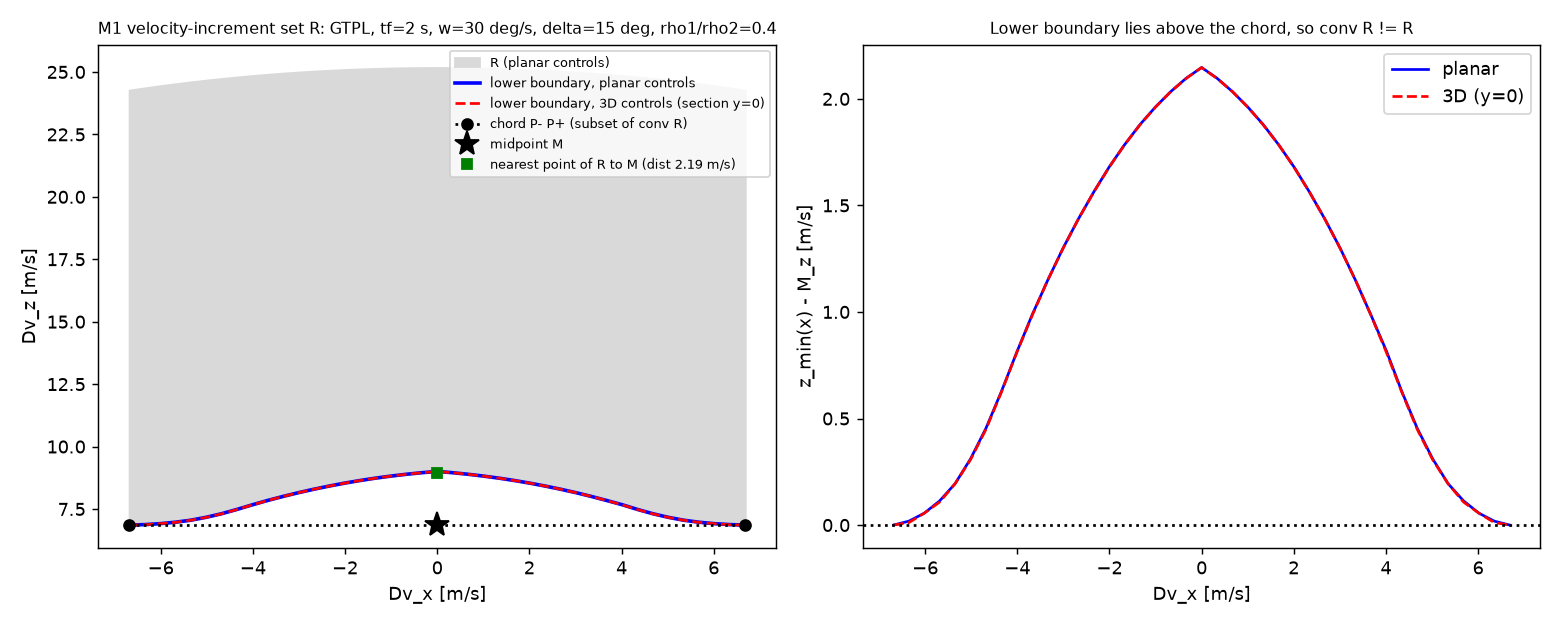
\includegraphics[width=\linewidth]{figures/t1_R_section.png}
\caption{Velocity-increment set $R$ of model M1 ($t_f=2$~s, $\omega=30^\circ$/s, $\delta=15^\circ$, $\rho_1/\rho_2=0.4$). The lower boundary
lies strictly above the chord $P_{-u}P_u$, so $M\in\conv R\setminus R$ (\cref{thm:B}). Planar and 3-D controls give the same boundary.
Numerical (inner discretization).}\label{fig:Rsection}
\end{figure}
\begin{figure}[t]\centering
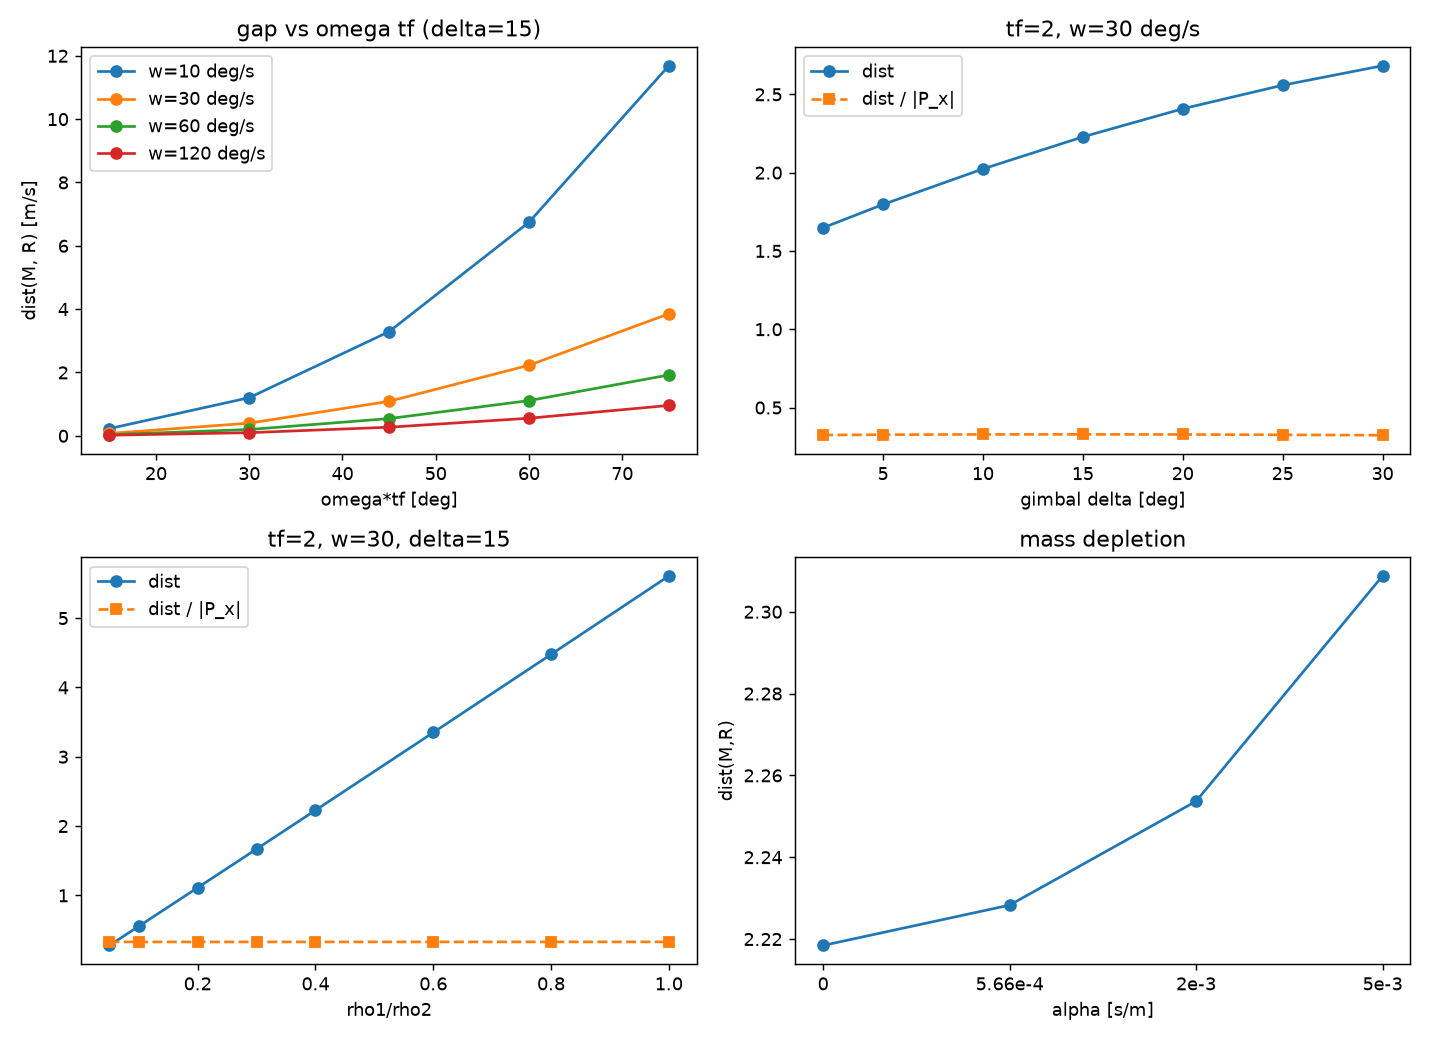
\includegraphics[width=.85\linewidth]{figures/t1_gap_sweeps.png}
\caption{Midpoint gap $\dist(M,R)$ against $\omega t_f$, $\delta$, $\rho_1/\rho_2$ and $\alpha$. The normalized gap $\dist/|P_x|$ is
flat in $\delta$ and $\rho_1/\rho_2$. Numerical.}\label{fig:gaplaw}
\end{figure}

\subsection{Beyond the proven regimes (no state constraints)}
For long horizons without a tilt cap the generalized midpoint gap grows (2.1/13.5/18.6~m/s at $t_f=2/4/8$~s), but that
regime uses inverted flight. With a $30^\circ$ tilt cap it is 1.15/1.56/0.35~m/s, shrinking as azimuthal sliding along the
cap weakens rigidity. In the tent variant the gaps are 0.66~m/s ($t_f=2$) and 6.24~m/s ($t_f=5$). For free final time the
Theorem~B witness, which starts underground, becomes reachable at a longer horizon (\cref{fig:freetf}). This is why the
free-final-time results need B$^*$ and a window. The torque-coupled TVC model M3 has nonconvex $R$ with gaps of 0.8--8~m/s
at $t_f=4$~s, and every minimizer of $\Delta v_z$ has nonzero lateral component.

\begin{figure}[t]\centering
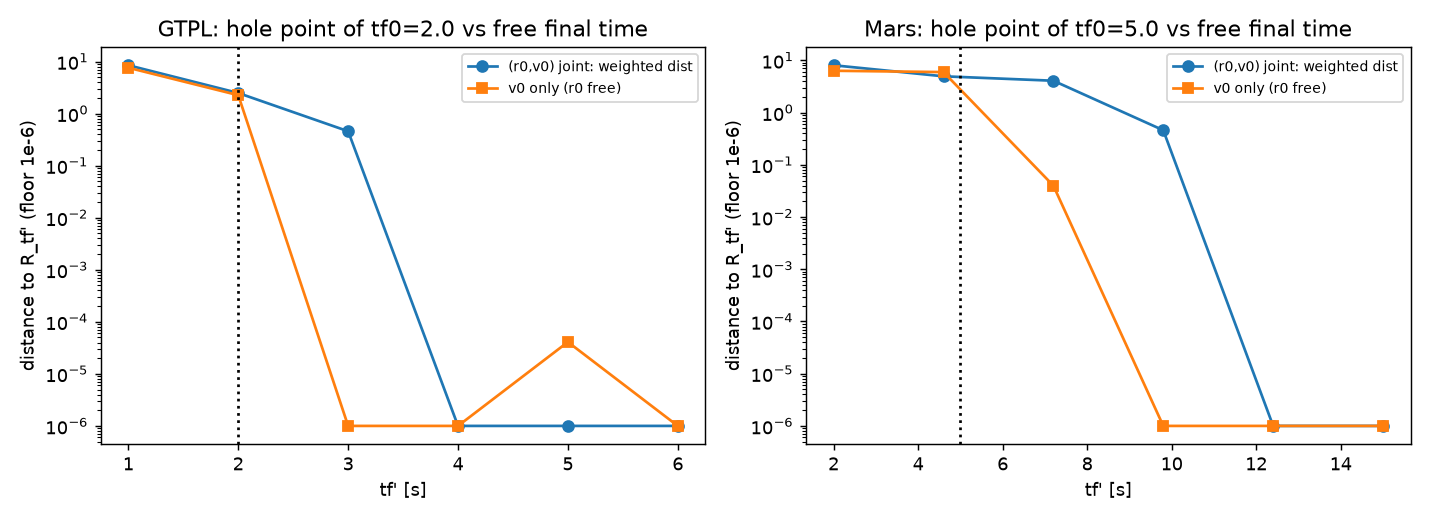
\includegraphics[width=.8\linewidth]{figures/t2_free_tf.png}
\caption{Free final time: the Theorem~B hole point at $t_f=2$~s (an underground datum) is reached at horizons $t_f'\ge4$~s. The
free-final-time obstruction therefore needs the dive-then-brake face and a compact window (\cref{cor:LS}). Numerical.}\label{fig:freetf}
\end{figure}

\subsection{With altitude constraints: the physically relevant sets}
Gaps of physically admissible data, all with $r_z(t)\ge0$ at every node, are summarized in \cref{tab:gaps}.
\begin{itemize}[leftmargin=*,itemsep=2pt]
\item \emph{B$^*$ face.} The rotation-midpoint gap is about $0.010$ (weighted m/s) at $t_f=4$~s and $0.007$ at $t_f=8$~s, stable in
$N$. That is real but tiny, roughly 0.3--0.5\% of the face's lateral velocity, consistent with \cref{rem:thin}.
\item \emph{Slice lemma (S) at dive-then-brake data.} Strict gaps of 0.016~m ($t_f=4$) and 0.009~m ($t_f=8$), with optimizers landing
1.5--2.4~m off axis. Coning narrows planar gaps by at most about 30\% (\cref{fig:slice}).
\item \emph{Face scan and the hop instance.} Among rotation-invariant vertical faces of $F^{\X}$, the pure-dive face is pinned at
$r_{0z}=0$, $v_{0z}>0$: a vehicle on the pad moving upward. Its midpoint gap is 0.65 ($t_f=4$) and 2.94 ($t_f=8$) weighted m/s,
about 65 ($t_f=4$) and 400 ($t_f=8$) times the B$^*$ gap. At pad data $r_0=0$, $v_{0,h}=0$, $t_f=4$~s, the landing-offset set $L$ is an annulus whose inner
radius grows from 0 to $4.99$~m as $v_{0z}$ goes from 7.65 to 7.90~m/s (\cref{fig:annulus}). Inside the window
$v_{0z}\in(7.727,7.917]$, landing back on the pad is infeasible while landing 0.5--8~m away is feasible. For the torque-coupled TVC
model at $v_{0z}=8.0$~m/s the pad lies 1.74~m from $L$. The \emph{rigorous} part of the hop result is an exact reduction, an
upright pad-landing limit $v_{0z}\le7.2045$ ($\alpha=0$) / $7.2833$ ($\alpha>0$), and explicit planar witnesses landing 6.58~m /
4.61~m off the pad at $v_{0z}=7.7116$ / $7.7425$. The \emph{hole} itself is not proved: quadratic and S-procedure certificates are
provably too loose here.
\item \emph{Tilt-rate-only model MT.} At the same hop data, $L$ is a full disk of radius 10.1~m. The full-direction rate limit, which
creates rigidity, is what creates the hole.
\item \emph{In-air descent.} From $r_0=(0,0,50)$~m, $v_0=(4,0,-5)$~m/s, $t_f=7$~s, the set $L$ is 104~m wide with no dent above
solver noise ($\le0.016$~m).
\item \emph{Long horizons and coning.} On the pure-dive face with a $30^\circ$ tilt cap, the 3-D slice gap falls to 0.69/0.50/0.106~m/s
at $t_f=8/12/20$~s (planar: 0.70/0.80/0.82), and at $t_f=20$~s the optimizer cones through $359^\circ$ on the cap. Coning fills
about 87\% of capped dents, but not all of them.
\item \emph{Pure TVC, upright at rest.} Full rigid body, $\pm15^\circ$ box gimbal at $100^\circ$/s from centred, mass depletion, roll free,
$r_z\ge0$, upright at rest at touchdown, face $\ell=r_{0z}+s^*v_{0z}$: the zero-lateral optimum lies below the free optimum by
$1.26\times10^{-2}$~m ($t_f=3$~s, $s^*=0.75$~s), $4.8\times10^{-3}$~m ($t_f=5$~s, $s^*=0.5$~s), $2.8\times10^{-2}$~m ($t_f=5$~s, $s^*=1$~s) and
$3.3\times10^{-2}$~m ($t_f=7$~s, $s^*=1$~s). The rigorous counterpart is \cref{thm:TVC1} (constant mass, unlimited gimbal rate; $t_f=1,2$~s uncapped, $3,5$~s capped).
\end{itemize}

\begin{table}[t]\centering\small
\caption{Size of the nonconvexity at physically admissible data ($r_z\ge0$), motivating vehicle. All entries numerical (upper bounds on true
distances, uncertified global optima) except where marked.}\label{tab:gaps}
\begin{tabular}{@{}llll@{}}\toprule
Face / instance & Model & $t_f$ [s] & Gap \\\midrule
B$^*$ face, rigorous bound (\cref{thm:Bstar}) & M1 & 7 & $\ge1.1\times10^{-5}$ (proved) \\
B$^*$ face, rotation midpoint & M1 & 4 / 8 & $\approx0.010$ / $0.007$ (weighted m/s) \\
Slice (S), dive-then-brake & M1 & 4 / 8 & 0.016 / 0.009 m in $\ell$; offsets 1.5--2.4 m \\
Pure-dive face (hop, $r_{0z}=0$) & M1 & 4 / 8 & 0.65 / 2.94 (weighted m/s) \\
Hop landing-set hole & M1 & 4 & up to 4.99 m \\
Hop landing-set hole & M3 (TVC) & 4 & 1.74 m \\
Dive-then-brake, upright at rest & PT (6-DOF) & 3 / 5 / 7 & 0.013 / 0.028 / 0.033 m \\
Same, certified (\cref{thm:TVC1}; const.\ mass) & PT (6-DOF) & 1 / 2 & $\ge9.6\times10^{-6}$ / $9.2\times10^{-5}$ m (proved) \\
Same, tilt-capped class, certified & PT (6-DOF) & 3 / 5 & $\ge4.8\times10^{-5}$ / $2.3\times10^{-6}$ m (proved) \\
In-air descent (50 m, $-5$ m/s) & M1 & 7 & none detected ($\le0.016$ m) \\\bottomrule
\end{tabular}
\end{table}

\begin{figure}[t]\centering
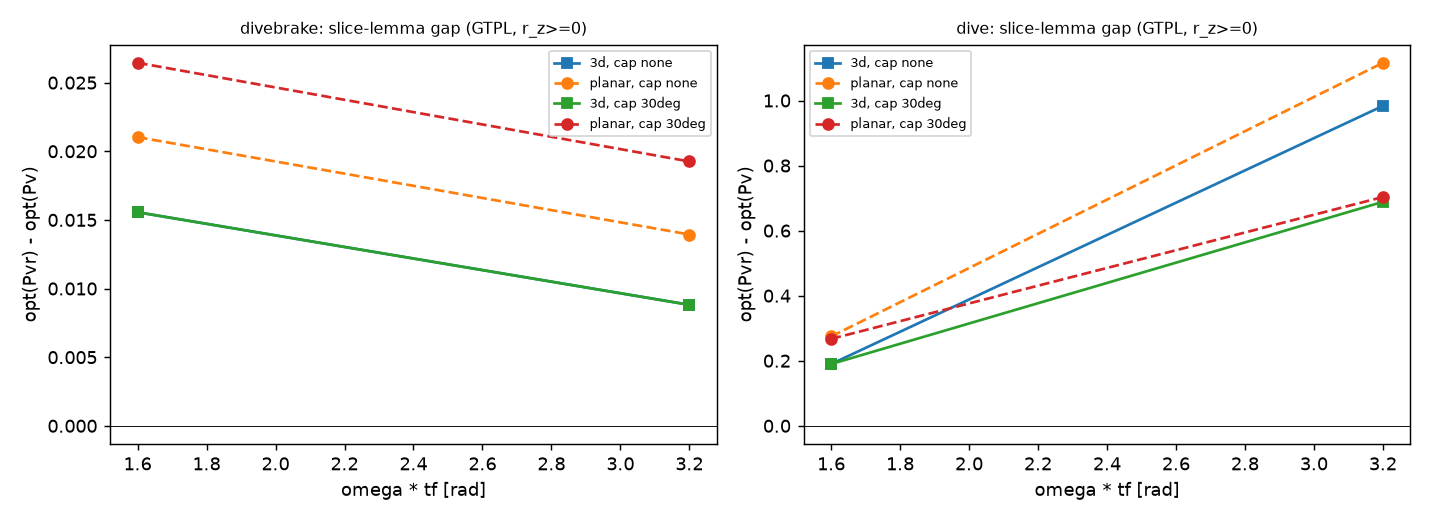
\includegraphics[width=.85\linewidth]{figures/s1_slice.png}
\caption{Slice-lemma gaps $\mathrm{opt}(P_{vr})-\mathrm{opt}(P_v)$ under $r_z\ge0$ for the dive-then-brake face (left; metres in $\ell$) and the
pure-dive face (right; m/s), planar versus 3-D (coning), with and without a $30^\circ$ tilt cap. A strictly positive gap means that the
straight-below landing is infeasible while an offset landing is feasible. Numerical.}\label{fig:slice}
\end{figure}
\begin{figure}[t]\centering
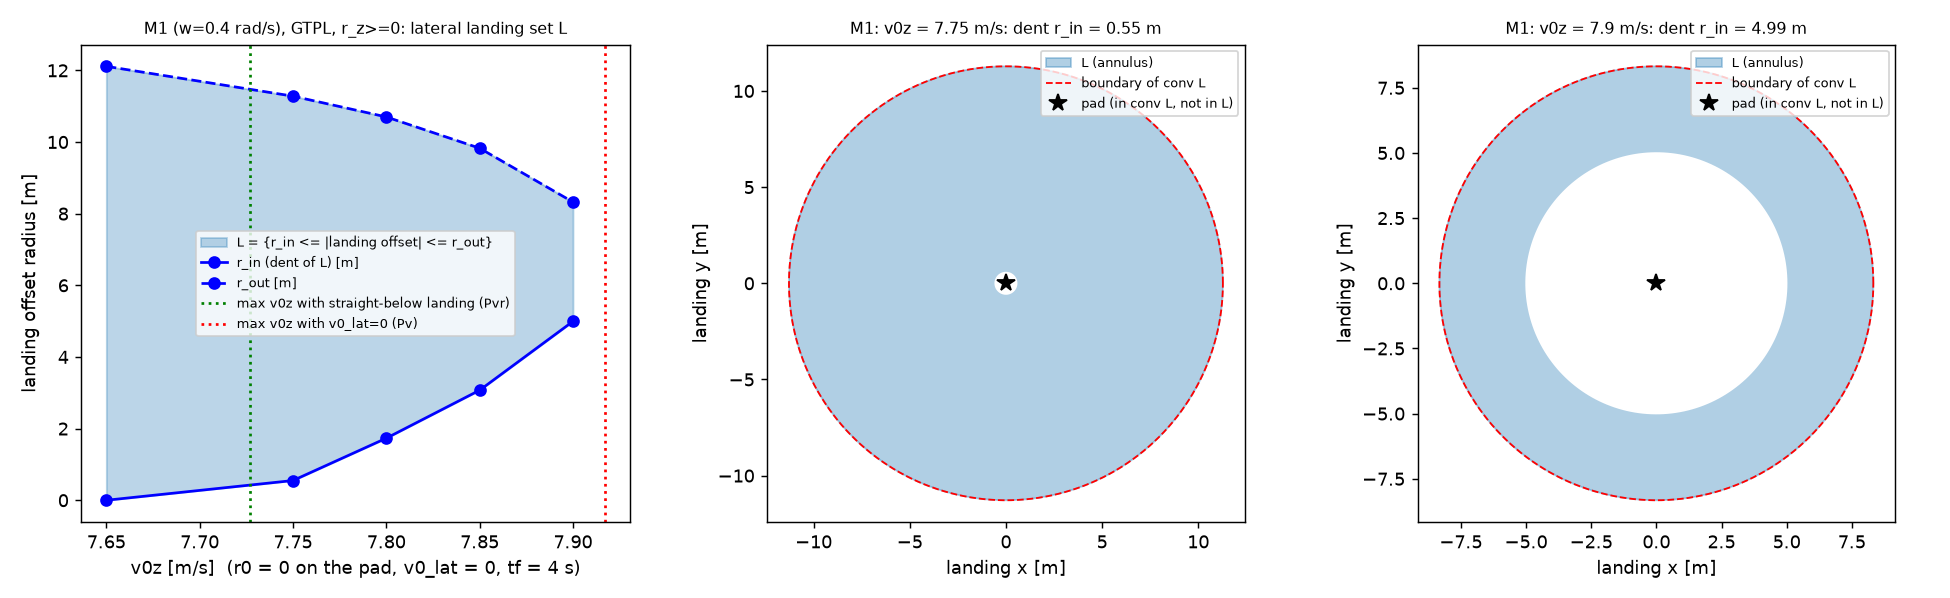
\includegraphics[width=\linewidth]{figures/s5_annulus.png}
\caption{Pad-launched hop ($r_0=0$, $v_{0,h}=0$, $t_f=4$~s, M1, $r_z\ge0$): the reachable landing-offset set $L$ is an annulus. The pad lies in
$\conv L$ but not in $L$ once $v_{0z}\gtrsim7.73$~m/s. By Theorem~D every state-linear relaxation of the minimum-landing-error problem reports
error $0$ at such data. Numerical; the hole is not certified.}\label{fig:annulus}
\end{figure}

\subsection{What 3-DOF LCvx asks of the vehicle}
The current guidance stack of the motivating vehicle solves a 3-DOF LCvx SOCP and hands only the thrust magnitude to the attitude
tracker. Its stored solutions contain thrust-direction jumps of $14.8^\circ$ within 24~ms and $180^\circ$ azimuth flips at
zero-order-hold switches. These demand roughly $10^3$~rad/s$^2$, against 1--3.5~rad/s$^2$ available. The relaxation is also not tight
on the stored minimum-throttle arc (296~N delivered against $\sigma m=400$~N), consistent with \cref{thm:CS}, which places lossiness at
minimum throttle. Together with \cref{thm:C6} (an upright body has effective cone $0$), this shows that the 5-DOF/6-DOF coupling is a
first-order issue for this vehicle, independent of the size of the nonconvexity.
